\section{Special Relativity}


\subsection{Introduction}

Here we are going to introduce mass-energy equivalence relation.

In physics, mass–energy equivalence is the relationship between mass and energy as by equation~\ref{eqn:E} in a system's rest frame, where the two values differ only by a constant and the units of measurement.The principle is described by the physicist Albert Einstein's famous formula.~\cite{Einstie}

\begin{equation}
	E=mc^2
	\label{eqn:E}
\end{equation}

The formula defines the energy E of a particle in its rest frame as the product of mass (m) with the speed of light squared ($c^2$). Because the speed of light is a large number in everyday units (approximately $3 \times 10 ^8$ meters per second), the formula implies that a small amount of rest mass corresponds to an enormous amount of energy, which is independent of the composition of the matter. Rest mass, also called invariant mass, is the mass that is measured when the system is at rest.


\subsection{Spacetime}

In physics, spacetime is any mathematical model which fuses the three dimensions of space and the one dimension of time into a single four-dimensional manifold. Spacetime diagrams can be used to visualize relativistic effects, such as why different observers perceive differently where and when events occur. In figure~\ref{f1:spacetime}.~\cite{Einstie}

\begin{figure}[h]
	\begin{center}
		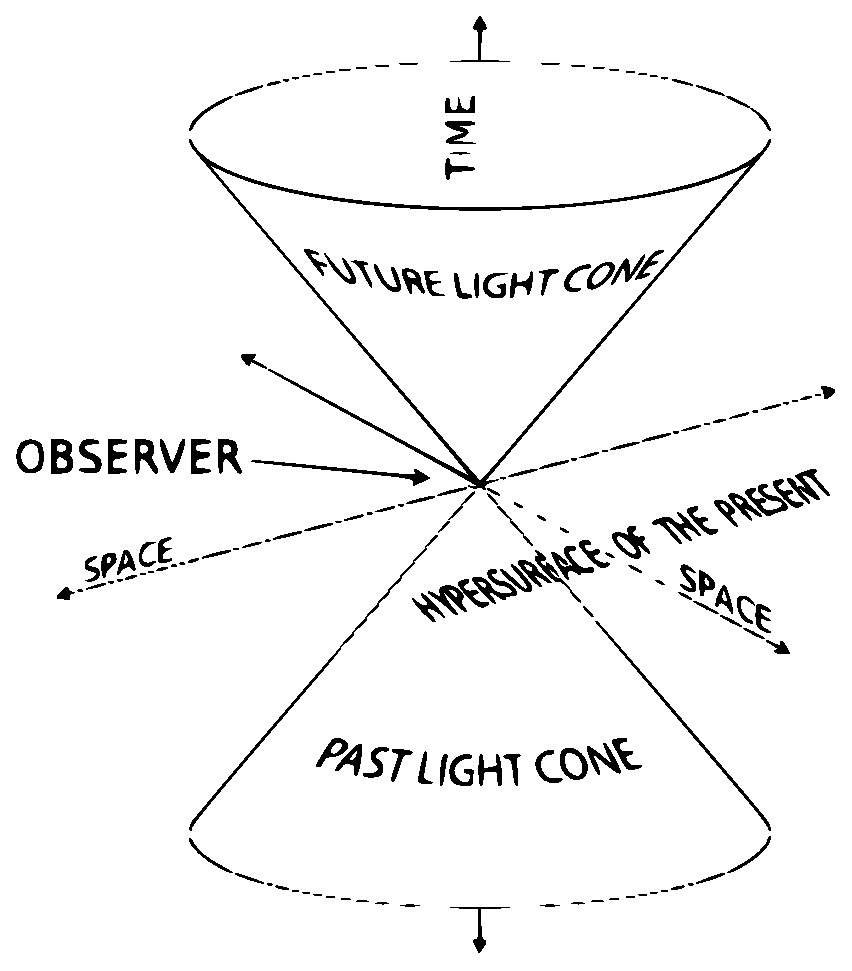
\includegraphics[scale=0.4]{ME20B166.eps}
	\end{center}
	\caption{The world line:a diagrammatic representation of spacetime}
	\label{f1:spacetime}
\end{figure}

